\section{The surrogate model}

\subsection{Overview}

This section presents the training process that have led to the description and definition of the target surrogate model, given a ready to use dataset, and the desired characteristics.

This is a straightforward example of regression problems, aiming to predict some output features from the input features, given a number of training example in a dataset. This is a typical machine learning problem, and is be addressed accordingly.

Initially, the performance of different methods are measured and the best one is selected. Then, a model is trained and evaluated, forming the core surrogate model.

\subsection{Machine learning methods}

This subsection assesses some of the most common machine learning algorithms for regression problems \cite{machine-learning-class}.

\subsubsection{K nearest neighbors}

In this context, the K-nearest neighbors (k-NN) methods is among one of the easiest to implement, using tools like the \href{https://scikit-learn.org/stable/modules/neighbors.html\#nearest-neighbors-regression}{scikit-learn} \cite{scikit-learn} module in python. Indeed, these simply require a single parameter value $k$ and output the average value of the output features of the $k$ nearest neighbors, computing a distance on the input features.

This features the drawback of not being able to learn quick variations in the outputs, as the averaging over the nearest sample points will filter out high frequency variations.

Results obtained with k-NN for various values of $k$ are shown in Table \ref{tab:results-knn}.

\begin{table}[h]
    \centering
    \begin{tabular}{|l|l|}
        \hline
        k & Validation error \\ \hline
        4  & 0.05082837 \\
        5  & 0.051765025 \\
        6  & 0.047083396 \\
        7  & 0.046183977 \\
        8  & 0.049501333 \\
        9  & 0.049218103 \\
        10 & 0.04949624 \\
        11 & 0.05036374 \\
        12 & 0.050881956 \\
        13 & 0.05243453 \\
        14 & 0.052941263 \\
        15 & 0.05362743 \\
        16 & 0.05440363 \\ \hline
    \end{tabular}
    \caption{Results obtained with k-NN}
    \label{tab:results-knn}
\end{table}

The optimal performance is achieved when $k$ is set to 7. Decreasing values of $k$ lead to an increase in error due to overfitting, whereas increasing values of $k$ result in higher errors attributed to underfitting.
% The best performance is obtained for $k$ equal to 7. Smaller values increase the error due to overfitting, while larger values suffer from underfitting, resulting in larger errors.

\subsubsection{Decision trees}

Decision trees, along with extremely randomized trees \cite{extremely-randomized-trees} are easy to implement\footnote{Again, using \href{https://scikit-learn.org/stable/modules/ensemble.html\#forests-of-randomized-trees}{scikit-learn}} machine learning methods as well, as they also involve a constrained and fixed number design parameters.

These methods, however, exhibit the limitation of producing piecewise constant output, and as stated above, it is required to be able to represent significantly fast variations in the output. Although it is possible to mimic using many successive steps, being peicewise constant will now introduce non linearities in the outputs, that is, unwanted steps in the prediction.

Results obtained with decision trees are shown in Table \ref{tab:trees-results}.

\begin{table}[h]
    \centering
    \begin{tabular}{|c|c|}
        \hline
        Number of trees & Validation error \\ \hline
        25  & 0.02385 \\
        35  & 0.02347 \\
        45  & 0.02275 \\
        55  & 0.02342 \\
        65  & 0.02361 \\
        75  & 0.02272 \\
        85  & 0.02360 \\
        95  & 0.02255 \\
        105 & 0.02294 \\
        115 & 0.02379 \\
        125 & 0.02263 \\
        135 & 0.02232 \\
        145 & 0.02317 \\ \hline
    \end{tabular}
    \caption{Results obtained with random forests}
    \label{tab:trees-results}
\end{table}

The highest accuracy is achieved with 135 trees. However in this case, the results are not as straightforward as for the k-NN technique, that showed a monotonic decrease, the minimum then an increase. As randomness is involved when choosing the splits when building the trees, the results are subject to a slight variance, inducing less obvious results. However, after 145 trees, the error starts steadily increasing.

These performance are higher than those of the nearest neighbors method, but not as strong as the following techniques.

\subsubsection{XGBoost}

XGBoost is currently one of the most popular machine learning technique \cite{XGBoost}. It actually is an efficient implementation of a machine learning method, tree boosting.

Boosting aims to construct a string predictive model from so-called weak learners, which in this case, are trees. Each learner is trained on the error of the output of the previous model, so that the previous output plus the newly trained learner output is a better prediction of the target output. Moreover, the samples are weighted in favor of the ones that were badly predicted by the previous model, in order to make sure we correct past mistakes.

In tree boosting, the main hyper-parameters are:
\begin{itemize}
    \item the number $n$ of weak learners stacked
    \item the \textit{learning rate}, a constant factor applied to the target difference (target output minus previous model output)
    \item the maximum depth of the weak learners
\end{itemize}

Resulting performance for some values of the hyper-parameters are reported in Table \ref{tab:results-xgboost}.

XGBoost's results are really good, achieving at best around 0.006 mean squared error on the validation set. This is not surprising given that this technique is quite popular in the literature. 

It is important to note that the method was tested over a previous version of the dataset (the one produced in \cite{carlas-thesis}) and not on the one generated in this thesis because the results were not yet available. The performance metrics should however not very dramatically between the former and the latter version of the dataset.
% Actually, for the first testing stage where the dataset created in this work was not available, the dataset from C. Vidal's work has been used as a first test. In this context, the results obtained with XGBoost outperformed the best neural network architecture.

\begin{table}[h!]
    \centering
    \begin{tabular}{|l|l|l|l||l|l|l|l||l|l|l|l|}
        \hline
        d & lr   & n    & err      & d  & lr   & n    & err      & d & lr   & n    & err      \\ \hline
        3 & 0.03 & 10   & 0.5248   &  4 & 0.1  & 10   & 0.1564   & 5 & 0.2  & 10   & 0.03299  \\
        3 & 0.03 & 20   & 0.3367   &  4 & 0.1  & 20   & 0.04522  & 5 & 0.2  & 20   & 0.01088  \\
        3 & 0.03 & 50   & 0.1100   &  4 & 0.1  & 50   & 0.01059  & 5 & 0.2  & 50   & 0.007287 \\
        3 & 0.03 & 100  & 0.033627 &  4 & 0.1  & 100  & 0.007168 & 5 & 0.2  & 100  & 0.006907 \\
        3 & 0.03 & 200  & 0.01294  &  4 & 0.1  & 200  & 0.006018 & 5 & 0.2  & 200  & 0.006681 \\
        3 & 0.03 & 500  & 0.007804 &  4 & 0.1  & 500  & 0.005489 & 5 & 0.2  & 500  & 0.006624 \\
        3 & 0.03 & 1000 & 0.006434 &  4 & 0.1  & 1000 & 0.005325 & 5 & 0.2  & 1000 & 0.006623 \\
        3 & 0.03 & 2000 & 0.005553 &  4 & 0.1  & 2000 & 0.005294 & 5 & 0.2  & 2000 & 0.006623 \\
        3 & 0.1  & 10   & 0.1886   &  4 & 0.2  & 10   & 0.04046  & 6 & 0.03 & 10   & 0.4870   \\
        3 & 0.1  & 20   & 0.06469  &  4 & 0.2  & 20   & 0.01313  & 6 & 0.03 & 20   & 0.2861   \\
        3 & 0.1  & 50   & 0.01586  &  4 & 0.2  & 50   & 0.007588 & 6 & 0.03 & 50   & 0.06760  \\
        3 & 0.1  & 100  & 0.009350 &  4 & 0.2  & 100  & 0.006579 & 6 & 0.03 & 100  & 0.01544  \\
        3 & 0.1  & 200  & 0.007291 &  4 & 0.2  & 200  & 0.006219 & 6 & 0.03 & 200  & 0.007516 \\
        3 & 0.1  & 500  & 0.005978 &  4 & 0.2  & 500  & 0.006029 & 6 & 0.03 & 500  & 0.006548 \\
        3 & 0.1  & 1000 & 0.005558 &  4 & 0.2  & 1000 & 0.006007 & 6 & 0.03 & 1000 & 0.006381 \\
        3 & 0.1  & 2000 & 0.005375 &  4 & 0.2  & 2000 & 0.006007 & 6 & 0.03 & 2000 & 0.006343 \\
        3 & 0.2  & 10   & 0.059425 &  5 & 0.03 & 10   & 0.4916   & 6 & 0.1  & 10   & 0.1368   \\
        3 & 0.2  & 20   & 0.02037  &  5 & 0.03 & 20   & 0.2894   & 6 & 0.1  & 20   & 0.03335  \\
        3 & 0.2  & 50   & 0.009474 &  5 & 0.03 & 50   & 0.07119  & 6 & 0.1  & 50   & 0.008382 \\
        3 & 0.2  & 100  & 0.007554 &  5 & 0.03 & 100  & 0.01647  & 6 & 0.1  & 100  & 0.006850 \\
        3 & 0.2  & 200  & 0.006287 &  5 & 0.03 & 200  & 0.006834 & 6 & 0.1  & 200  & 0.006594 \\
        3 & 0.2  & 500  & 0.005976 &  5 & 0.03 & 500  & 0.005326 & 6 & 0.1  & 500  & 0.006504 \\
        3 & 0.2  & 1000 & 0.005935 &  5 & 0.03 & 1000 & 0.005069 & 6 & 0.1  & 1000 & 0.006491 \\
        3 & 0.2  & 2000 & 0.005894 &  5 & 0.03 & 2000 & 0.004952 & 6 & 0.1  & 2000 & 0.006491 \\
        4 & 0.03 & 10   & 0.5013   &  5 & 0.1  & 10   & 0.1425   & 6 & 0.2  & 10   & 0.0302   \\
        4 & 0.03 & 20   & 0.3042   &  5 & 0.1  & 20   & 0.03577  & 6 & 0.2  & 20   & 0.01046  \\
        4 & 0.03 & 50   & 0.08414  &  5 & 0.1  & 50   & 0.008340 & 6 & 0.2  & 50   & 0.007929 \\
        4 & 0.03 & 100  & 0.02168  &  5 & 0.1  & 100  & 0.006145 & 6 & 0.2  & 100  & 0.007743 \\
        4 & 0.03 & 200  & 0.008364 &  5 & 0.1  & 200  & 0.005640 & 6 & 0.2  & 200  & 0.007651 \\
        4 & 0.03 & 500  & 0.005841 &  5 & 0.1  & 500  & 0.005433 & 6 & 0.2  & 500  & 0.007622 \\
        4 & 0.03 & 1000 & 0.005203 &  5 & 0.1  & 1000 & 0.005371 & 6 & 0.2  & 1000 & 0.007622 \\
        4 & 0.03 & 2000 & 0.004922 &  5 & 0.1  & 2000 & 0.005371 & 6 & 0.2  & 2000 & 0.007622 \\ \hline
    \end{tabular}
    \caption{Results for some values of the XGBoost parameters. The learning rate is labelled "lr", the maximum depth "d" and the number of estimators n, while the validation error is denoted by "err".}
    \label{tab:results-xgboost}
\end{table}

The best performance is observed with a maximum depth of 4, a learning rate set to 0.03 and 2000 trees. Further fine-tuning may slightly improve this value, in particular reduce the learning rate and increase the number of trees even more, but further investigation showed that the performance stagnate starting from 1800.

% As there are tree dimensions to take into account, we need to find combination of values. Results in Table \ref{tab:results-xgboost} indicate that there is a balance to find between the depth of the approximators and their number. Sh

\subsubsection{Kernel-based methods\label{section:kernel-methods}}

One might consider applying a kernel method with one of the other method mentioned above. While this may indeed improve the quality of the resulting model, and also solve the issue that was representing fast changes in the output, nevertheless, finding a suitable kernel is a difficult.

Since there is no ready-to-use kernel for this specific case, and that finding such a kernel would be a hard task, kernel methods are discarded.

\subsubsection{Artificial neural network}

Artificial neural networks (ANN) are used in this work to build our surrogate model. These types of methods offer a large flexibility, due to their entirely customizable architecture, as well as a large learning capacity. This makes them able to modelize with good accuracy some complex, non-linear functions.

In most recent applications of these ANNs, a lot of different strategies are used to process the data efficiently. For example, convolutional layers convey a lot of meaning in the context of image processing, or transformers are well suited to process sequences \cite{deep-learning-class}.

In this case, the inputs boils down to the 6 variables values, listed in Table \ref{table:reference-values}. There are no patterns in this data, because even if their actual values were correlated in some way, the simulations dataset we have as an input at this stages has its input features drawn from a latin hypercube sampling, meaning they have a fixed, very low correlation. This correlation originates from the fact that the sampling aims at optimizing the design space coverage, not from a meaningful, exploitable source.

Thus, a simple multi-layer perceptron (MLP) architecture is chosen, and the next requirement is to describe the characteristics of that MLP, that are:
\begin{itemize}
    \item The number of layers
    \item The numbers of neurons in each layers
    \item The activation function at each layer
\end{itemize}

Some experiments are run to provide some baselines for getting a first approximation of what performs well. These results are presented in Table \ref{tab:nn-results}.

\begin{table}[h!]
    \centering
    \begin{tabular}{|p{0.7\textwidth}|p{0.2\textwidth}|}
        \hline
        Architecture & Validation error \\ \hline
        (180, 'relu', 0.4), (100, 'tanh', 0.4) & 0.00484 \\
        (180, 'relu', 0.4), (100, 'tanh', 0.4) & 0.00499 \\
        (180, 'relu', 0.4), (100, 'tanh', 0.4) & 0.00480 \\
        (70, 'relu', 0.5), (70, 'relu', 0.5) & 0.04538 \\
        (100, 'relu', 0.4), (100, 'relu', 0.4) & 0.02506 \\
        (100, 'relu', 0.5), (100, 'relu', 0.5) & 0.04111 \\
        (100, 'relu', 0.6), (100, 'relu', 0.6) & 0.04481 \\
        (100, 'relu', 0.7), (100, 'relu', 0.7) & 0.10410 \\
        (80, 'relu', 0.7), (80, 'relu', 0.7) & 0.06514 \\
        (150, 'relu', 0.6), (100, 'relu', 0.6) & 0.02693 \\
        (250, 'relu', 0.4), (125, 'relu', 0.4) & 0.01295 \\
        (200, 'relu', 0.5), (125, 'relu', 0.5) & 0.01734 \\
        (200, 'relu', 0.5), (125, 'tanh', 0.5) & 0.00532 \\
        (200, 'relu', 0.4), (125, 'tanh', 0.4) & 0.00555 \\
        (200, 'relu', 0.4), (100, 'tanh', 0.4) & 0.00581 \\
        (150, 'relu', 0.45), (100, 'tanh', 0.45) & 0.00585 \\
        (150, 'relu', 0.5), (100, 'tanh', 0.5) & 0.00603 \\
        (150, 'relu', 0.4), (80, 'tanh', 0.4) & 0.00597 \\
        (220, 'relu', 0.5), (125, 'relu', 0.5) & 0.01086 \\
        (250, 'relu', 0.5), (125, 'relu', 0.5) & 0.02421 \\
        (250, 'tanh', 0.4), (125, 'tanh', 0.4) & 0.04193 \\
        (200, 'relu', 0.5), (150, 'relu', 0.5), (100, 'relu', 0.4) & 0.07372 \\
        (120, 'relu', 0.4), (120, 'relu', 0.4), (120, 'relu', 0.4) (120, 'relu', 0.4), (80, 'relu', 0.4) & 0.12163 \\
        (50, 'relu', 0.3), (50, 'relu', 0.3), (50, 'relu', 0.3), (50, 'relu', 0.3) & 0.08267 \\
        (50, 'relu', 0.4), (50, 'relu', 0.4), (50, 'relu', 0.4), (50, 'relu', 0.4) & 0.14292 \\
        (50, 'relu', 0.2), (50, 'relu', 0.2), (50, 'relu', 0.2) & 0.02622 \\
        (50, 'relu', 0.2), (50, 'relu', 0.2), (50, 'relu', 0.2), (50, 'relu', 0.2) & 0.05221 \\
        (50, 'relu', 0.3), (50, 'relu', 0.3), (50, 'relu', 0.3) & 0.05723 \\
        (50, 'relu', 0.4), (50, 'relu', 0.4), (50, 'relu', 0.4) & 0.08706 \\
        (150, 'relu', 0.5), (150, 'relu', 0.5), (150, 'relu', 0.5) & 0.07769 \\
        (150, 'relu', 0.5), (100, 'relu', 0.5), (100, 'relu', 0.5) & 0.08809 \\
        (150, 'relu', 0.5), (150, 'relu', 0.5), (100, 'relu', 0.5) & 0.08098 \\
        (200, 'relu', 0.5), (200, 'relu', 0.5), (150, 'relu', 0.5) & 0.07682 \\
        (190, 'relu', 0.5), (190, 'relu', 0.5), (140, 'relu', 0.5) & 0.06489 \\
        (200, 'relu', 0.5), (200, 'relu', 0.5), (150, 'relu', 0.5), (30, 'relu', 0.3) & 0.08749 \\
        (200, 'relu', 0.5), (200, 'relu', 0.5), (150, 'relu', 0.5), (50, 'relu', 0.3) & 0.09094 \\
        (200, 'relu', 0.5), (200, 'relu', 0.5), (200, 'relu', 0.5) & 0.07010 \\
        (150, 'relu', 0.5), (150, 'relu', 0.5), (150, 'relu', 0.5), (150, 'relu', 0.5) & 0.13490 \\ \hline
    \end{tabular}
    \caption{Results for some architectures of neural networks. Architectures are formatted as a list of layers, which are written as ($n$, $a$, $p$) tuples, where $n$ is the number of neurons, $p$ the dropout value and $a$ the activation function}
    \label{tab:nn-results}
\end{table}

These result outperform every other method. The fact that different but close architecture show similar performance brings some confidence about the reproducibility: the random initialization of the weights in the network could have led to an exceptionally good model. Moreover, several runs of the same architecture yield similar ouputs, validating this intuition.

It is worth mentioning that some larger network architecture, \textit{e.g.} $(300, 'relu', 0), (300, 'relu', 0),$ $(200, 'relu', 0)$ achieved really good results, even slightly better than the best one. However these were not implementing dropout, so that they are high changes of being subject to overfitting. If dropout is added, the observed performance decrease, confirming the overfitting hypothesis.

This is why the relative smallness of the network is a strength, as it will also act against overfitting, as having fewer parameters leaves less room for learning noise.

\subsubsection{Selection of the machine learning technique and parametrization}

In the end, neural networks are opted for. They benefit from the best performance in terms of mean squared error on the validation test, but neural networks MLPs also present the following advantages:
\begin{itemize}
    \item They are relatively lightweight, in comparison to the K-nearest neighbors methods, that needs to store the entire dataset, and the randomized trees, that need to store its trees structures. Neural networks only needs their weights that are fairly small with this few input variables.
    \item Grasp non-linear behaviour with accuracy
\end{itemize}

Preliminary experiments basically consist in the test undertaken to assess the performance of different architectures (reported in Table \ref{tab:nn-results}). While the firsts steps of testing used another dataset that available at the time, ultimately the generated dataset was the only one in use for this assessments.

The architecture is selected as the optimal one among baselines, and is provided in Table \ref{tab:nn-layers}. While hyper-parameter tuning may have produced another result, the latter could potentially suffer from overfitting, as described above. 

\begin{table}[h!]
    \centering
    \begin{tabular}{|l|l|l|}
        \hline
        Layer index & Layer type & Weights count \\ \hline
        1 & Fully connected linear layer, 6 inputs to 180 outputs & $6\times 180 = 1080$ \\
        2 & ReLU activation function & 0 \\
        3 & Dropout layer, with $p=0.4$ & 0 \\
        4 & Fully connected linear layer, 180 inputs to 100 inputs & $180\times 100=18000$ \\
        5 & $\tanh$ activation function & 0 \\
        6 & Dropout layer, with $p=0.4$ & 0\\
        7 & Fully connected linear layer, 100 inputs to 2 outputs & $100\times 2$ \\ \hline
    \end{tabular}
    \caption{Description of the layers of in the selected architecture for the model}
    \label{tab:nn-layers}
\end{table}

Consequently, the final parameterization of the model involves the setting of all its weights, that lie in layers 1, 4 and 7. The total count of parameters adds up: $1080 + 18000 + 200 = 19280$.

\subsection{Machine learning aspects}

\subsubsection{Validation and testing\label{ssec:val-testing}}

In machine learning, validation and testing are crucial steps in order to ensure the performance of a model. To implement these, one must separate the data into three sets.

\begin{itemize}
    \item The validation set is used for hyperparameters tuning. Given its influence on the model, it can introduce bias into the model.
    \item The test set is used to evaluate the model's performance, on unseen data.
    \item The training set is used to train the model.
\end{itemize}

% Typically, the data is split into three subsets. However, in this setting, the training, input data comes from a latin hypercube, and can be generated. Taking this into account, one may then consider the use of different LHS.
Typical machine learning applications dispose of a single, fixed dataset, that has to be split to constitute three desired sets. However, in this context, we can inexpensively run sets of simulations to obtain more data points, from another LHS. It is interesting to consider generating more than a single dataset from a unique LHS.

For the training set, joining different sets drawn with LHS is not expected to improve performance. As the LHS are independent of each other, there is a great chance to draw samples that are really close to each other, or worse, equal, what the LHS aims to avoid.

On the other hand, using a set drawn from a different LHS (than the one used for the training set) for testing and validation is interesting. This will provide data that spans the whole input space, but not yet exactly the same as the data used for training. Thanks to the input space coverage, the evaluation made at testing will be more extensive, and thanks to being independent of the training data, this evaluation should remain unbiased. 

Conversely, the validation set being sampled from a LHS now providing a guarantee that it spans the whole space could make the work of the learning agent easier, giving it access to each of the LHS sample from the training set.

However promising, this approach will not be done in this work, to ensure that the unbiased property of the trained model persists, and that the term "validation error" keeps the exact same meaning as in the literature.

\subsubsection{Overfitting}

An inherent challenge to machine learning methods is the overfitting, or its opposite, underfitting. These terms refer to the cases where the training is respectively too specific to the training data, and not enough specific.

Overfitting is a result of excessive learning, leading to learning some noise or some particularities of the dataset, while underfitting means that there is not enough learning, so that the model is not able to represent all the cases, even the one that are well represented in the available data.

The main tool used to prevent it in a neural network is the dropout. During the training phases, each neuron on a layer will have some probability $p$, typically between 0.3 and 0.5, of being set to 0, independently of its value. This methods ensures that the network will not be excessively relying on some neurons in its output. During testing oviously, the dropout is removed and all neurons are functional.

\subsubsection{Underfitting}

On the other hand, underfitting means there is not enough learning happening. For example, a neural network with only 2 neurons corresponding to the ouputs could not learn any non-linear functions, with some tweaks due to the eventual activation function.

In this setting, although underfitting is still a shortfall, it is not regarded as bad as the overfitting. The latter introduces errors that come from noise that is completely random, inevitably introducing imprecisions. But we keep in mind that the target to be approximated, that are outputs from the Dispa-SET model, are themselves an approximation, though accurate, of the reality. So if these are subject to some bias or imperfections, the best model would learn them as well.

Because an underfitting model of the dataset created using Dispa-SET would still be a decent estimate of the reality, which is the primary objective in this context, underfitting is preferable to overfitting.

These will have to be assessed during training to ensure the validity of the model.

\subsubsection{Bias\label{ssec:bias}}

An other source of imprecision in machine learning is the bias. This relates to the fact that there exist some noise in the data, that cannot be filtered out, or imprecisions in the assumptions, that inevitably conducts to noise in the output.

However, in this setting, there is very little one could implement to reduce its significance. First, the data points have been drawn from a latin-hypercube sampling strategy, that precisely aims at spreading the samples equitably all over the input space. Then, the output features were computed from a Dispa-SET run on this sample.

Hence, the primary source of bias that can be addressed pertains to model training inaccuracies resulting from suboptimal model design.

The other plausible source of bias is the simulation made in Dispa-SET. Of course, Dispa-SET is also itself a model, thus relying on some assumptions and subject to its own modelling of the reality. And as such, it may introduce a bias in its computations, that will necessarily be learned by the surrogate model. But there is no way to assess this bias, and obviouly Dispa-SET itself focuses on making that bias as negligible as possible.

This consideration is of interest, as Dispa-SET has multiple formulations, namely LP and MILP, that then have different bias with respect to reality.

\subsection{Training}

\subsubsection{Implementation}

All the files for this section lie in the \texttt{nn} folder.

The implementation of the training process comprises the following files:
\begin{itemize}
    \item \texttt{config.py}, that holds all the high-level specifications of the training, such as the names of the outputs, the train-test-validation set ratios, the number of epochs etc.
    \item \texttt{model.py}, that contains the function building the model, thus the definition of the neural network's architecture.
    \item \texttt{baselines.py}, that contains code to train models with pre-defined architectures, in order to quickly and easyly have an overview of the order of magnitude involved.
    \item \texttt{train.py}, that contains the code for the hyperparameter tuning and model training.
    \item \texttt{view.py}, that contains the utilities to visualize the results.
    \item \texttt{tests.py}, that contains the testing of the other machine learning methods (k-NN, trees, XGBoost)
    \item \texttt{data}, \texttt{logs}, \texttt{models} directories, that contain the datasets, the runs' logs, and the trained models respectively.
\end{itemize}

\subsubsection{Results}

The selected architecture is a two-layer network:
\begin{enumerate}
    \item 180 neurons, ReLU activation, 0.4 chance of dropout
    \item 100 neurons, hyperbolic tangent activation, 0.4 chance of dropout
\end{enumerate}

The mean squared error over the training epochs is shown in Figure \ref{fig:nn-validation-error-curve}.

\begin{figure}[h]
    \centering
    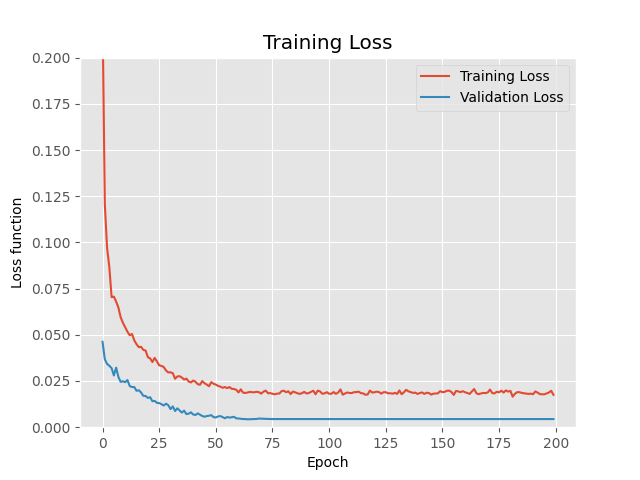
\includegraphics[width=0.7\textwidth]{resources/images/mse-finalarch.png}
    \caption{Mean squared error on the validation set}
    \label{fig:nn-validation-error-curve}
\end{figure}

The occurrence of overfitting appears unlikely, as evidenced by the trend observed in Figure \ref{fig:nn-validation-error-curve}, wherein the validation error exhibits no notable increase beyond a certain number of training epochs. This pattern contrasts with the ongoing reduction in training error.
% Overfitting is not likely, because as can be seen in Figure \ref{fig:nn-validation-error-curve}, the validation error never increases significantly after a given amount of learning epochs, while the training error is still decreasing. An example of such obvious overfitting is shown in Figure \ref{fg:overfitting}.

\begin{figure}[h]
    \centering
    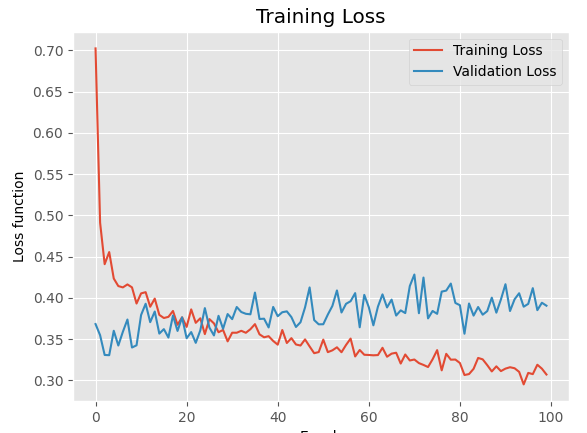
\includegraphics[width=0.6\textwidth]{resources/images/overfitting.png}
    \caption{An (unrelated) example of clear overfitting, the validation loss increasing after some time}
    \label{fig:overfitting}
\end{figure}

\subsubsection{Observations \label{ssec:surrogate-model-surf-observations}}

To further confirm the absence of overfitting in this result, the \texttt{view.py} file is used to browse across the multi-dimensional function, with surface plots.

These plots draw one of the outputs against two of the inputs, keeping the four other inputs constant. These constant values are summarized in Table \ref{tab:default-view-values}. Attention should be paid to the scale of the plots, as these do not start at 0.

\begin{table}[h!]
    \centering
    \begin{tabular}{|c|c|}
        \hline
        Input name & Value \\ \hline
        Capacity ratio & 1.15 \\
        Share flexibility & 0.5 \\
        Share storage & 0.25 \\
        Share wind & 0.25 \\
        Share PV & 0.25 \\
        rNTC & 0.35 \\ \hline
    \end{tabular}
    \caption{Default values for constant inputs. These are the middle of their base interval, see Table \ref{table:reference-values}}
    \label{tab:default-view-values}
\end{table}

Several surfaces are depicted in Figure \ref{fig:all-views}. The following observation are made from the latter illustrations.

\begin{figure}[h]
    \centering
    \begin{subfigure}[b]{0.49\textwidth}
        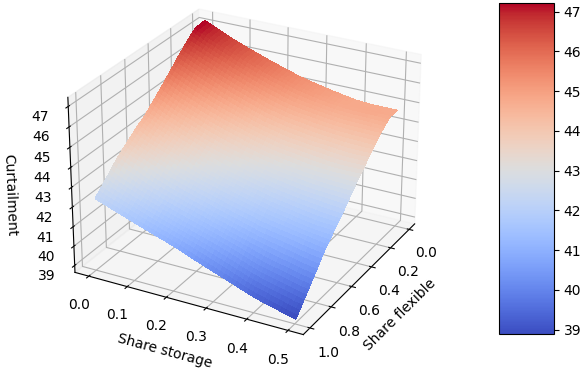
\includegraphics[width=\textwidth]{resources/images/view_1-2-0.png}
        \caption{Curtailment against share flexibility and share storage}
        \label{fig:surf-1-2-0}
    \end{subfigure}
    \hfill
    \begin{subfigure}[b]{0.49\textwidth}
        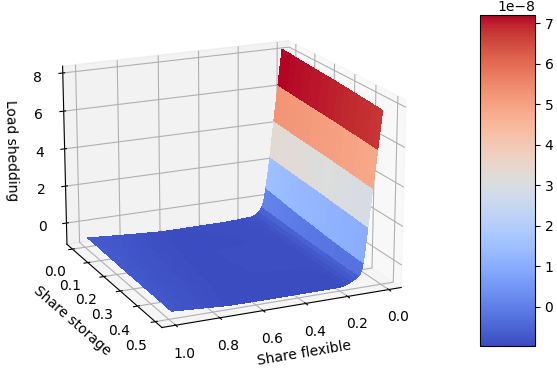
\includegraphics[width=\textwidth]{resources/images/view_1-2-1.png}
        \caption{Load shedding against share flexibility and share storage}
        \label{fig:surf-1-2-1}
    \end{subfigure}
    \hfill
    \begin{subfigure}[b]{0.49\textwidth}
        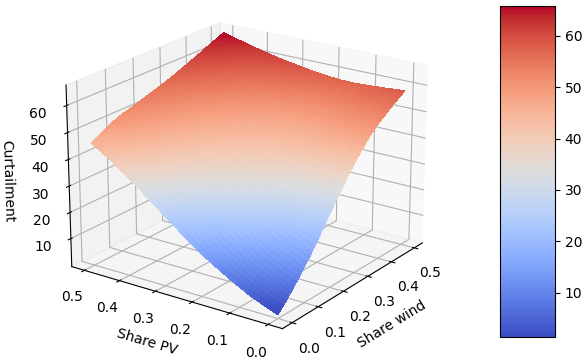
\includegraphics[width=\textwidth]{resources/images/view_3-4-0.png}
        \caption{Curtailment against share wind and share PV}
        \label{fig:surf-3-4-0}
    \end{subfigure}
    \hfill
    \begin{subfigure}[b]{0.49\textwidth}
        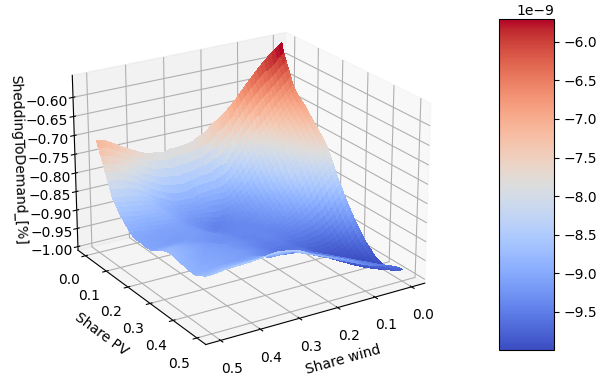
\includegraphics[width=\textwidth]{resources/images/view_3-4-1.png}
        \caption{Load shedding against share wind and share PV}
        \label{fig:surf-3-4-1}
    \end{subfigure}
    \hfill
    \begin{subfigure}[b]{0.49\textwidth}
        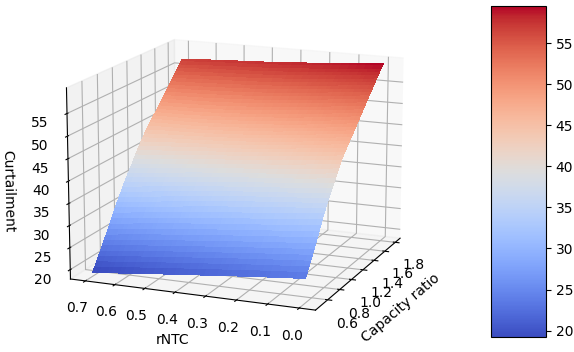
\includegraphics[width=\textwidth]{resources/images/view_0-5-0.png}
        \caption{Curtailment against capacity ratio and rNTC}
        \label{fig:surf-0-5-0}
    \end{subfigure}
    \hfill
    \begin{subfigure}[b]{0.49\textwidth}
        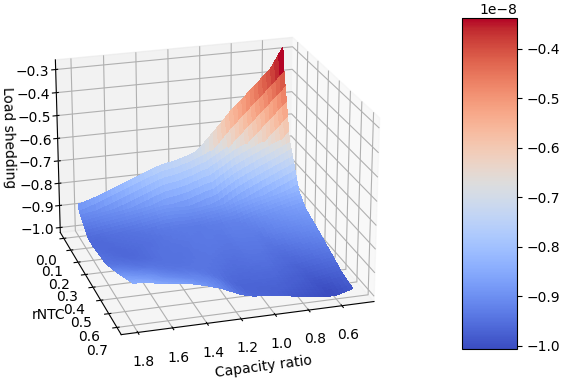
\includegraphics[width=\textwidth]{resources/images/view_0-5-1.png}
        \caption{Load shedding against capacity ratio and rNTC}
        \label{fig:surf-0-5-1}
    \end{subfigure}
    \caption{Different views of the multi-dimensional function, with four fixed inputs and two varying inputs.}
    \label{fig:all-views}
\end{figure}

\begin{itemize}
    \item Figure \ref{fig:surf-1-2-0} follows the natural intuition, as higher shares of storage units and flexible units both contribute to the reduction of the curtailment.
    \item Figure \ref{fig:surf-1-2-1} points out the crucial impact of the share of flexible units on the load shedding for small values. Naturally, when peaks in demand appear, if no unit is susceptible to be started, there is no other way than to cut the exceeding demand out.
    \item Figure \ref{fig:surf-3-4-0} also confirms the intuition, as it outlines the increase in curtailment with an increase of either share solar or share PV.
    \item Figure \ref{fig:surf-3-4-1} is the most intriguing one. First, it is noticed that the scale is the lower here. The most surprising part is that it features local minima, and that when the share PV is close to 0, the load shedding as a function of the share of wind energy is U-shaped. This phenomenon is hard to explain theoretically, the most likely cause remains a weak learning of the model.
    
    Moreover, the shape of the surface changes rapidly when changing the other constant values, therefore taking other values than disclosed in Table \ref{tab:default-view-values}, which validates the hypothesis of a weak learning.

    In comparison, the other surfaces do not move that significantly with similar change, coming down to a slight upwards or downwards shift, depending on the direction of the change, occasionnaly with a light amplitude change.
    \item Figure \ref{fig:surf-0-5-0} follows the intuition as well, but also highlights the stronger impact of the capacity ratio on the curtailment compared to the rNTC. This is not surprising, as the share of electricity import is not that huge. However, this may change dramatically depending on the country considered.
    \item Figure \ref{fig:surf-0-5-1} is interesting, as it shows that the load shedding grows when both the rNTC and capacity ratio lower. As low rNTC means little importation possible, and low capacity ratio not much margin to fulfill the demand, this actually makes sense.
\end{itemize}

% \subsection{Comparison with MEDEAS state of the art}

% Well, requires the surrogate model

% \mywarning{TODO}